\chapter{Programopbygning}

I dette kapitel vil programmets opbygning blive beskrevet. Først vil programmets arkitektur blive beskrevet, derefter navigeringen i programmets brugergrænseflade.


\section{Programopbygning}\label{sec:programopbygning}

\begin{figure}[h]
\centering
\tikzstyle{lille} = [rectangle, minimum width=2cm, minimum height=1.0cm,text centered, draw=black, fill=blue!30]
\tikzstyle{invi} = [draw, rectangle, minimum height=2cm, minimum width=2cm]
\tikzstyle{line} = [draw]
\tikzstyle{arrow} = [thick,->,>=stealth]
\begin{tikzpicture}[node distance = 1.5cm]
%noderne (objekterne) laves
\node (uixaml) [lille] {UI XAML};
\node (cb) [lille, below of=uixaml] {CB};
\node (invi1) [invi,draw=none,below of=cb] {};
\node (model) [lille, below of=invi1] {Model};
\node (idal) [lille, right of=invi1] {iDal};
\node (sqldal) [lille, right=0.5cm of idal] {SQLite Dal};
\node (efdal) [lille, below of=sqldal] {EF Dal};
\node (sql) [lille, right=0.5cm of sqldal] {SQLite};
\node (ef) [lille, below of=sql,align=center] {Entity\\ Framework};
%pointers laves
\draw [line] (uixaml) -- (cb);
\draw [line] (cb) -| (idal);
\draw [dashed] (cb)-- (model);
\draw [line] (model) -| (idal);
\draw [line] (idal) -- (sqldal);
\draw [line] (idal) to [bend right] (efdal);
\draw [line] (sqldal) -- (sql);
\draw [line] (efdal) -- (ef);
\end{tikzpicture}
\caption{Programopbygning: Figuren viser sammenhængen mellem de forskellige komponenter i programmet.}
\label{img:Program_flow}
\end{figure}
På \myref{img:Program_flow}, ses den overordnede struktur af programmet.
I bunden ses modelboksen, som repræsenterer modellaget.
Her findes de modeller vi anvender i programmet.
Modellerne er forbundet til vores Dal, Data Abstraction Layer, hvilket er den generiske kontakt fra programmet ud mod databasen.
Fra den generiske IDal findes der forbindelser ud til et SQLite Dal og et Entity Framwork Dal, som hver i sær har forbindelse til de databaser de hører til.
Ideen ved det generiske IDal er at der let kan skiftes mellem forskellige databaser, dette vil der kommes nærmere ind på i \myref{chap:database}.
Over IDal og Model findes code-behind og UI'en.
Code-behind og UI er forbundet da UI-filerne kun indeholder grafiske elementer og code-behind filerne indeholder det kode som UI'en har brug for til at fungere.
Code-behind filerne er også i direkte kontakt med IDal for at kunne tilgå data i databasen.
Yderligere har code-behind også kendskab til modellaget, illustreret med en stiplet linje.
Code-behind har behov for kendskab til modellerne, da der flere steder i koden har været brug for at instantiere modellerne for at håndetere data. 
\section{Navigering i programmet}
\begin{figure}[H]
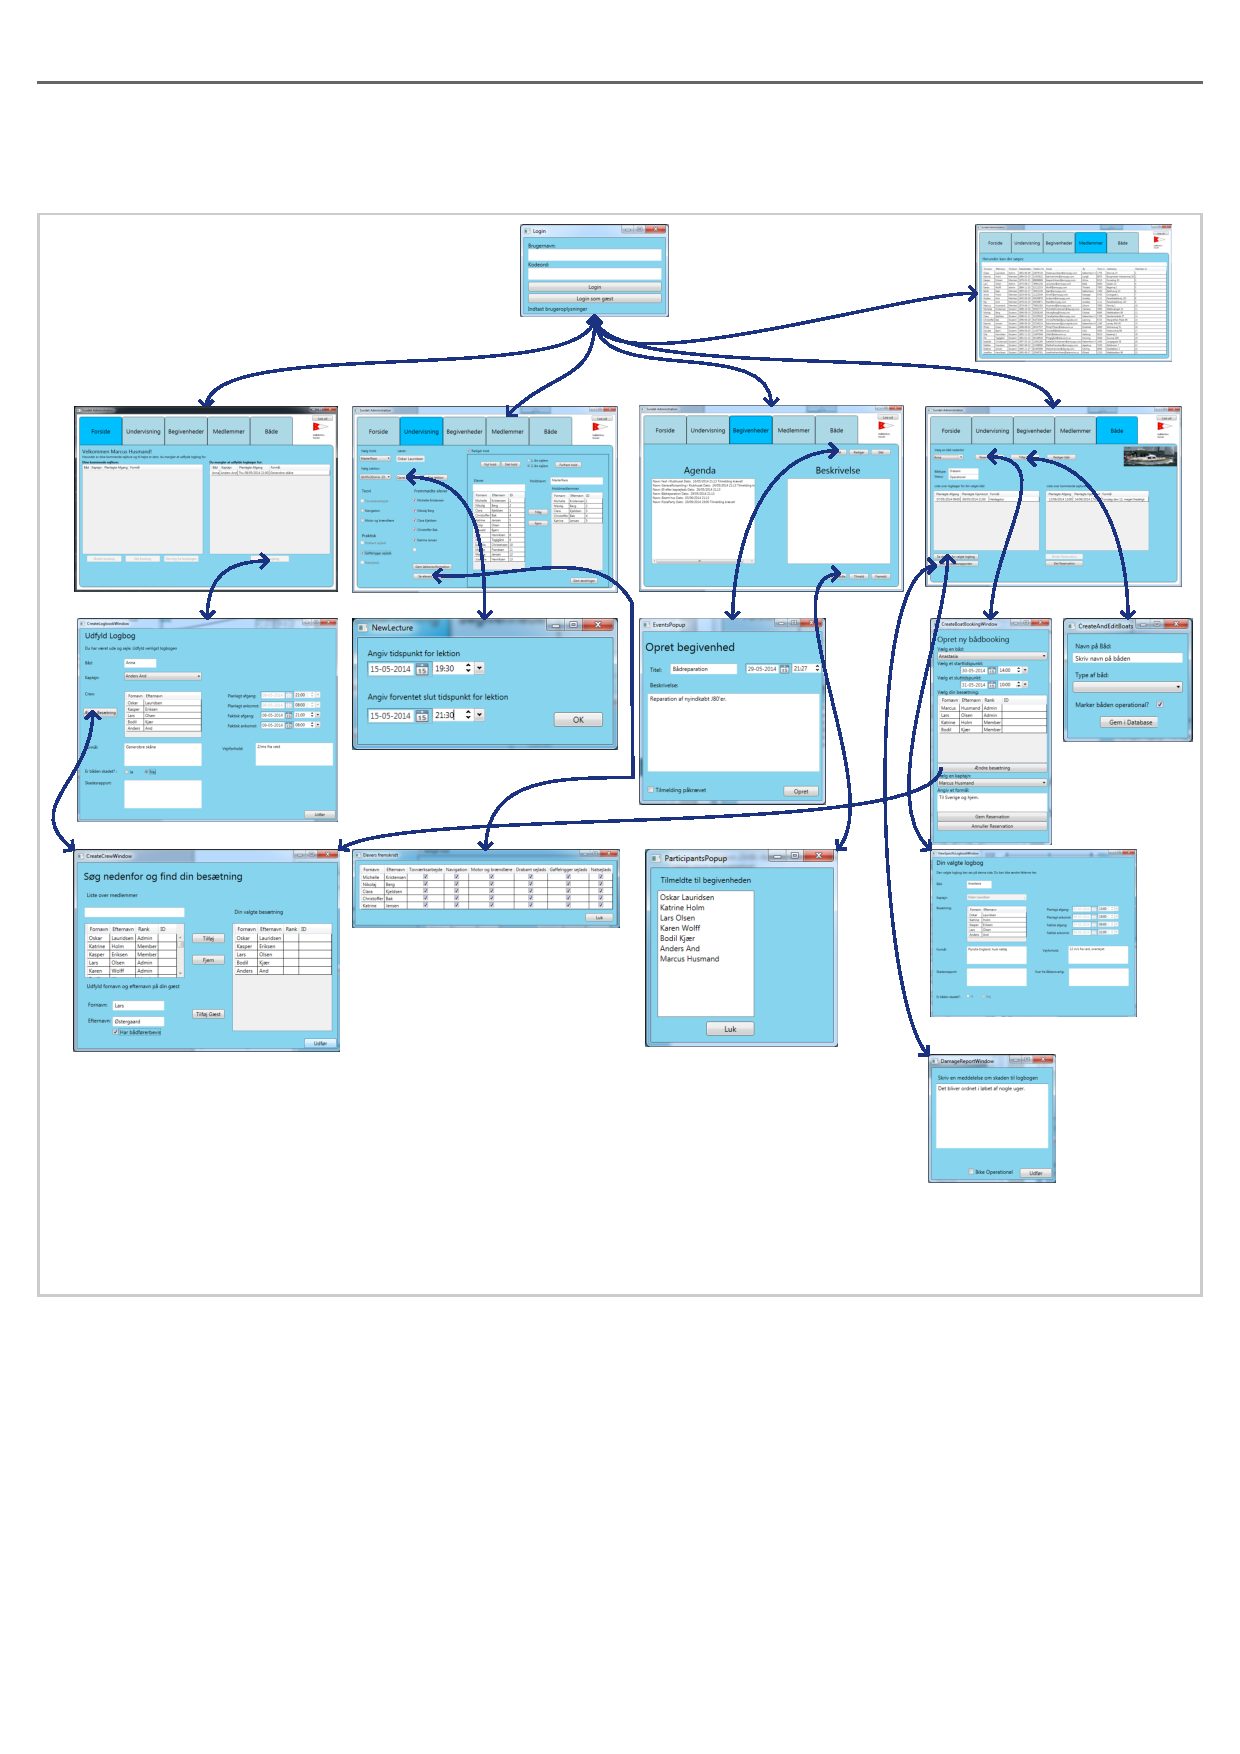
\includegraphics[width=1\textwidth]{UI/UI2.pdf}
\label{img:programNavigation}
\vspace{-310pt}
\caption{Navigations skema for programmet}
\vspace{-20pt}
\end{figure}
På \myref{img:programNavigation} ses der hvordan navigeringen i programmet foregår.
Øverst ses login-vinduet, herfra logger brugeren ind med sine login informationer, eller en gæst kan logge ind ved at trykke på \textit{login som gæst}-knappen.
Brugeren ser nu hovedvinduet, hvilket er vinduet i midten med 5 tabs i toppen.
Antallet af tabs variere alt efter hvilken position brugeren har i systemet, hvilket kan ses på \myref{tab:permissions}. 
Fra forside tabben kan der så navigeres til de andre tabs, som brugeren har tilgængelig.
Pilene illusterer de dialogbokse som brugeren kan åbne fra de forskellige tabs.
Dialogboksene åbnes ved at trykke på knapper inde i tabsne, fx under  \textbf{Bådreservation} kan opret booking dialogen åbnes ved at trykke på knappen \textit{Reserver Båden}. 
På samme måde åbnes de resterende dialoger ved tryk på knapper.
Flere steder i programmet anvendes de samme dialogvinduer, fx fra forsiden findes en mulighed for at ændre på en reservation, hvilket åbner en mindre modificeret udgave af booking dialogen, hvorfra at besætningsvælger dialogen også kan åbnes.
Desuden findes Logbogsdialogen også på forsiden.
Forskellen på logbogsdialogen på forsiden og den under bådreservation, er at dialogen under forsiden er lavet for at logbogen kan udfyldes, mens den under bådreservation er read-only.
\fxnote{Aner ikke om knapperne har de rigtige navne}
\fxnote{Billedet skal opdateres, mangler opret event,}